\documentclass{beamer}
\usetheme{Warsaw}  %% Themenwahl

\usepackage[utf8]{inputenc}
\usepackage[ngerman]{babel}
\usepackage{ngerman}
\usepackage{wrapfig}
\usepackage{multicol}

\graphicspath{{../}}
 
\title{Hashverfahren}
\author{Lars Schmertmann}
\date{\today}
 
\begin{document}
\maketitle
%\setcounter{tocdepth}{3}
%\frame{\tableofcontents}
%\frame{\tableofcontents[currentsection]}

\frame{ \begin{multicols}{2} \tableofcontents \end{multicols} }

\section{Eigenschaften}
  \begin{frame}
    \frametitle{Eigenschaften}
    Ein guter kryptographischer Hash zeichnet sich aus durch:\\
    ~\\
    \begin{itemize}
      \setlength{\itemsep}{20pt}
      \item Kollisionsresistent:
      \begin{itemize}
        \item schwer, $ x \neq y $ zu finden mit $ h(x) = h(y) $
      \end{itemize}
      \item Urbildresistent:
      \begin{itemize}
        \item schwer, zu einem $ a $ ein $ y $ zu finden mit $ a = h(y) $
      \end{itemize}
    \end{itemize}
    ~\\
    Gelingt es die Urbildresistenz zu umgehen,\\
    ist die Kollisionsresistenz ebenfalls umgangen.
  \end{frame}

\section{Komponenten von SHA256}
\subsection{Padding}
  \begin{frame}
    \frametitle{Padding}
    Auffüllen der Eingabe auf ein Vielfaches von 512 Bit.\\
    ~\\
    Allgemeines Padding:\\
    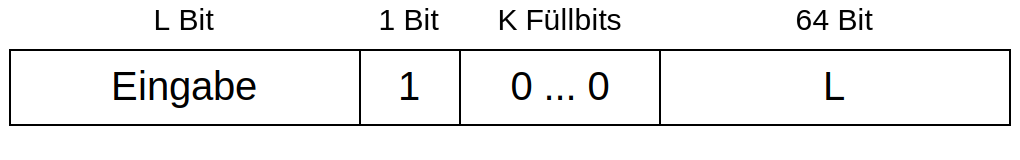
\includegraphics[width=300pt]{padding}\\
    \pause~\\
    Mögliche Lösung für SAT-Berechnung\\
    - Länge von 55 Byte vorgeben:\\
    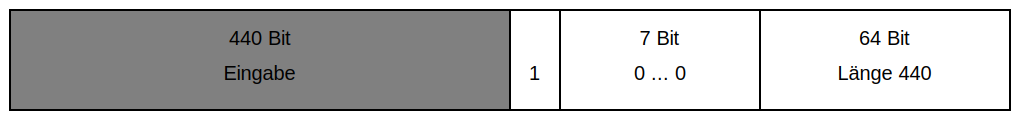
\includegraphics[width=300pt]{padding-allgemein}
  \end{frame}
\subsection{Funktionen}
  \begin{frame}
    \frametitle{Funktionen}
    \begin{itemize}
      \setlength{\itemsep}{20pt}
      \item Expansion
        \begin{itemize}
          \setlength{\itemsep}{10pt}
          \item $ SSIG0(x) = ROTR^{7}(x)~XOR~ROTR^{18}(x)~XOR~SHR^{3}(x) $
          \item $ SSIG1(x) = ROTR^{17}(x)~XOR~ROTR^{19}(x)~XOR~SHR^{10}(x) $
        \end{itemize}
      \item Computation
        \begin{itemize}
          \setlength{\itemsep}{10pt}
          \item $ CH( x, y, z) = (x~AND~y)~XOR~( (NOT~x)~AND~z) $
          \item $ MAJ( x, y, z) = (x~AND~y)~XOR~(x~AND~z)~XOR~(y~AND~z) $
          \item $ BSIG0(x) = ROTR^{2}(x)~XOR~ROTR^{13}(x)~XOR~ROTR^{22}(x) $
          \item $ BSIG1(x) = ROTR^{6}(x)~XOR~ROTR^{11}(x)~XOR~ROTR^{25}(x) $
        \end{itemize}
    \end{itemize}
  \end{frame}
\subsubsection{CH}
  \begin{frame}
    \frametitle{CH}
    $ CH( x, y, z) = (x~AND~y)~XOR~( (NOT~x)~AND~z) $\\
    ~\\
    $ c \Leftrightarrow (x \wedge y) \veebar ( \neg x \wedge z) $\\
    ~\\
    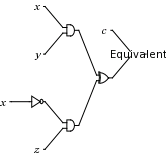
\includegraphics[scale=0.5]{ch.png}\\
    ~\\
    $ (\neg c \vee \neg x \vee y) \wedge (\neg c \vee x \vee z) \wedge (c \vee \neg x \vee \neg y) \wedge (c \vee x \vee \neg z) $
  \end{frame}
\subsubsection{MAJ}
  \begin{frame}
    \frametitle{MAJ}
    $ MAJ( x, y, z) = (x~AND~y)~XOR~(x~AND~z)~XOR~(y~AND~z) $\\
    ~\\
    $ m \Leftrightarrow (x \wedge y) \veebar (x \wedge z) \veebar (y \wedge z) $\\
    ~\\
    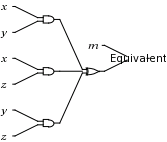
\includegraphics[scale=0.5]{maj.png}\\
    ~\\
    $ (\neg m \vee x \vee y) \wedge  (\neg m \vee x \vee z) \wedge (\neg m \vee y \vee z) \wedge $\\
    $ (m \vee \neg x \vee \neg y) \wedge (m \vee \neg x \vee \neg z) \wedge (m \vee \neg y \vee \neg z) $
    \end{frame}
\subsubsection{*SIG*}
  \begin{frame}
    \frametitle{*SIG*}
    $ *SIG*(a, b, c) = a~XOR~b~XOR~c $\\
    ~\\
    $ s \Leftrightarrow a \veebar b \veebar c $\\
    ~\\
    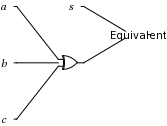
\includegraphics[scale=0.5]{sig.png}\\
    ~\\
    $ (\neg a \vee \neg b \vee \neg c \vee s) \wedge (\neg a \vee \neg b \vee c \vee \neg s) \wedge $\\
    $ (\neg a \vee b \vee \neg c \vee \neg s) \wedge (\neg a \vee b \vee c \vee s) \wedge $\\
    $ (a \vee \neg b \vee \neg c \vee \neg s) \wedge (a \vee \neg b \vee c \vee s) \wedge $\\
    $ (a \vee b \vee \neg c \vee s) \wedge (a \vee b \vee c \vee \neg s) $
  \end{frame}
\subsection{Vorbereitung}
  \begin{frame}
    \frametitle{Vorbereitung}
    Jeder Block der Länge 512 Bit wird auf 2048 Bit erweitert.\\
    ~\\
    Die zusätzliche Bits werden wie folgt generiert:\\
    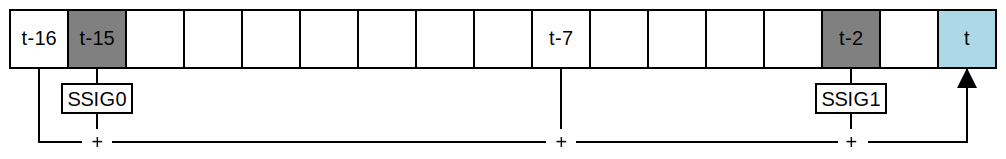
\includegraphics[width=300pt]{extend}
  \end{frame}
\subsection{Berechnung}
\subsubsection{Verfahren}
  \begin{frame}
    \frametitle{Verfahren}
    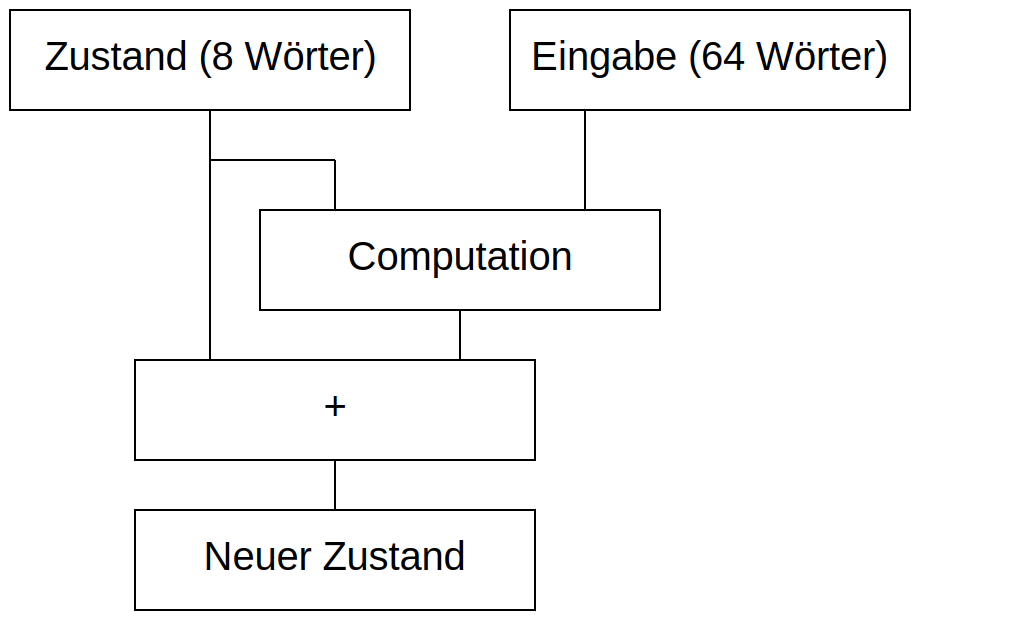
\includegraphics[width=300pt]{verfahren}
  \end{frame}
\subsubsection{Mischen}
  \begin{frame}
    \frametitle{Mischen}
    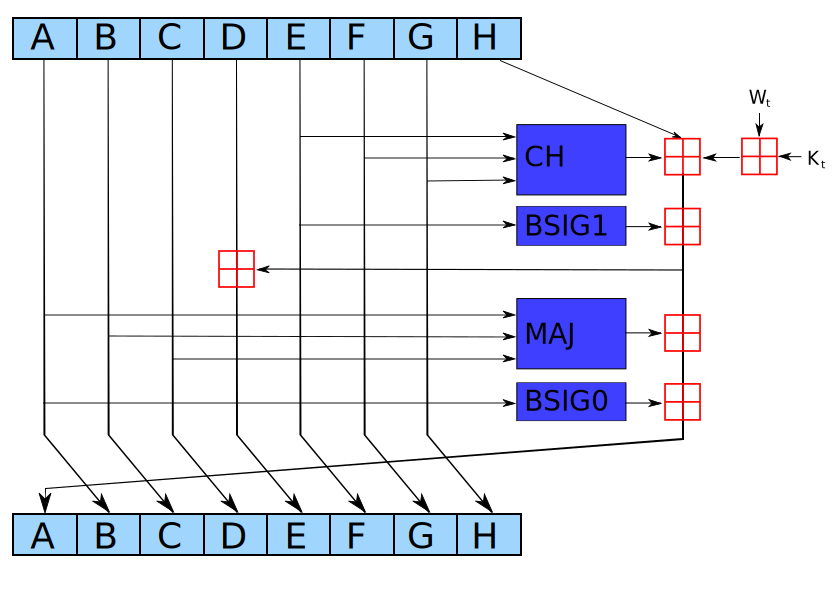
\includegraphics[width=300pt]{sha256}
  \end{frame}
\subsubsection{Kern}
  \begin{frame}
    \frametitle{Kern}
    \includegraphics[width=300pt]{sha25core}
  \end{frame}
\section{Bitcoin}
\subsection{Aufgabe}
  \begin{frame}
    \frametitle{Aufgabe}
    Aufbau eines Bitcoinblocks:
    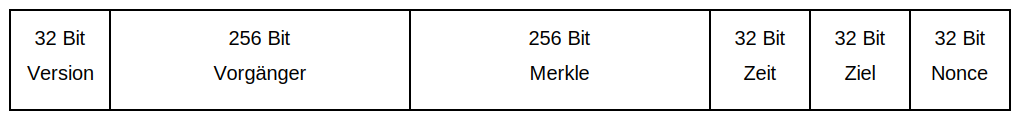
\includegraphics[width=300pt]{bitcoinblock}\\
    ~\\
    Aufgabe:\\
    Finde eine Nonce, so dass SHA256(SHA256(Block))\\
    kleiner als das aktuelle Ziel ist.\\
    ~\\
    Das bedeutet aktuell:\\
    Der Hashwert muss 67 führende Nullen haben.
  \end{frame}
\subsection{Padding}
  \begin{frame}
    \frametitle{Padding}
    Eingabe für die erste Hashberechnung:
    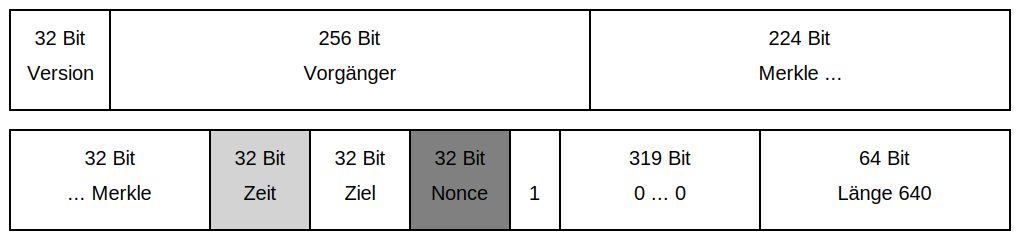
\includegraphics[width=300pt]{blockpadding}\\
    ~\\
    Eingabe für die zweite Hashberechnung:
    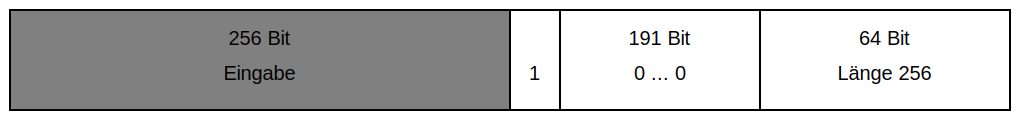
\includegraphics[width=300pt]{blockpadding2}\\
  \end{frame}
\section{Architektur}
\subsection{Modul}
  \begin{frame}
    \frametitle{Modul}
    \begin{wrapfigure}{l}{85pt}
    \fbox{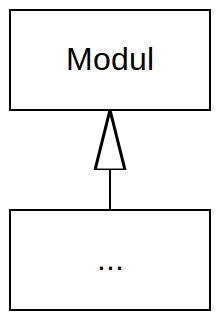
\includegraphics[width=75pt]{arch_modul}}
    %\caption{Bildbezeichnung}
    %\label{fig:bild}
    \end{wrapfigure}
    Basisklasse für alle Module.\\
    ~\\
    Stellt Funktionen für die Konfiguration\\
    und Erstellung der Grundgatter bereit.\\
    ~\\
    \texttt{Modul(bitWidth, inputCount, outputCount)}\\
    ~\\
    \texttt{virtual void create(Printer* printer) = 0;}\\
  \end{frame}
  \begin{frame}
    \frametitle{Modul}
    \begin{wrapfigure}{l}{85pt}
    \fbox{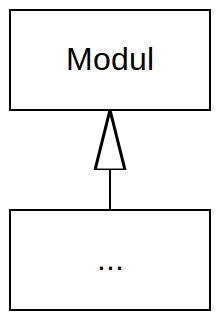
\includegraphics[width=75pt]{arch_modul}}
    %\caption{Bildbezeichnung}
    %\label{fig:bild}
    \end{wrapfigure}
    Bisher erstellte Grundmodule:\\
    ~\\
    Konstante, Addierer, BSIG0, BSIG1,\\
    SSIG0, SSIG1, MAJ, CH,\\
    ~\\
    Bisher erstellte komplexe Module:\\
    ~\\
    Addierer: Konstante, B0MAJ, B1CH, SSIG\\
    Vorbereitung, Vorbereitung48, Berechnung\\
  \end{frame}
\subsection{Printer}
  \begin{frame}
    \frametitle{Printer}
    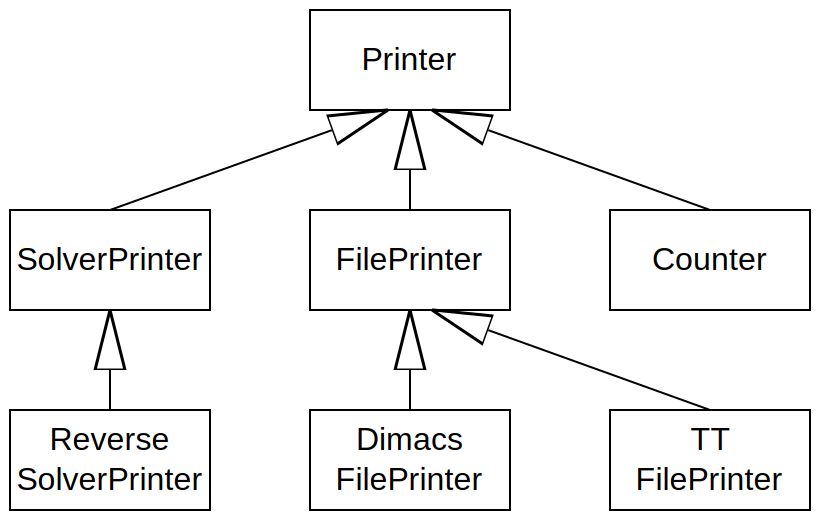
\includegraphics[width=250pt]{arch_printer}\\
    \texttt{virtual void create(bool xOR, const std::vector{\textless}CMSat::Lit{\textgreater}\& vars) = 0;}
  \end{frame}
  \begin{frame}
    \frametitle{KNF to TT}
    Verwendetes Encoding im TTFilePrinter:\\
    ~\\
    \begin{tabular}{lp{2cm}|cccc|c|}
       &  & \multicolumn{4}{c|}{Eingänge} & Ausgang\\
       &  & a & b & c & d & r \\
      \cline{3-7}
      $ \neg a \vee b \vee d $   &  & 1 & 0 & - & 0 & 0 \\
      $ b \vee c \vee \neg d $   &  & - & 0 & 0 & 1 & 0 \\
      $ a \vee b \vee c \vee d $ &  & 0 & 0 & 0 & 0 & 0 \\
      $ \neg b \vee \neg c $     &  & - & 1 & 1 & - & 0
    \end{tabular}
  \end{frame}
\section{Ergebnisse}
\subsection{CBMC vs Eigenbau}
  \begin{frame}
    \frametitle{CBMC vs Eigenbau}
    \begin{itemize}
      \item CBMC
      \begin{itemize}
        \item $ \sim $ 70.000 Variablen
        \item $ \sim $ 350.000 Klauseln
      \end{itemize}
      \item Eigenbau
      \begin{itemize}
        \item $ \sim $ 50.000 Variablen
        \item $ \sim $ 250.000 Klauseln
      \end{itemize}
      \item Eigenbau mit XOR
      \begin{itemize}
        \item $ \sim $ 50.000 Variablen
        \item $ \sim $ 150.000 Klauseln
      \end{itemize}
    \end{itemize}
  \end{frame}
\subsection{Sat-Solving}
  \begin{frame}
    \frametitle{Sat-Solving}
    \begin{itemize}
      \item SHA256 Vorwärtsberechnung funktioniert
      \item SHA256 Rückwärtsberechnung \newline funktioniert mit 18 von 64 Runden
      \begin{itemize}
        \item Mit 4 Threads in unter 5 Minuten. Nicht deterministisch.
      \end{itemize}
      \item Espresso - Nutzbar für CH und MAJ
      \begin{itemize}
        \item *SIG*: 64 Variablen: Zu komplex
      \end{itemize}
    \end{itemize}
  \end{frame}
\subsection{CC-Mining}
  \begin{frame}
    \frametitle{CC-Mining}
    \begin{itemize}
     \item Allgemeine Konfliktklausen errechnen
     \item Konfliktklausel ausdenken und Literale einzeln negiert in die SAT-Instanz einfügen: Falls nicht lösbar ist die Konfliktklausel gültig
     \item Bis 4 oder 5 Literalen machbar. Bei mehr Literalen gibt es zu viele Möglichkeiten
     \item Producer / Consumer: Eine Thread-Safe-Klasse die Aufgaben an beliebig viele Consumer vergibt.
    \end{itemize}
  \end{frame}
\subsection{Analyse}
  \begin{frame}
    \frametitle{Kern}
    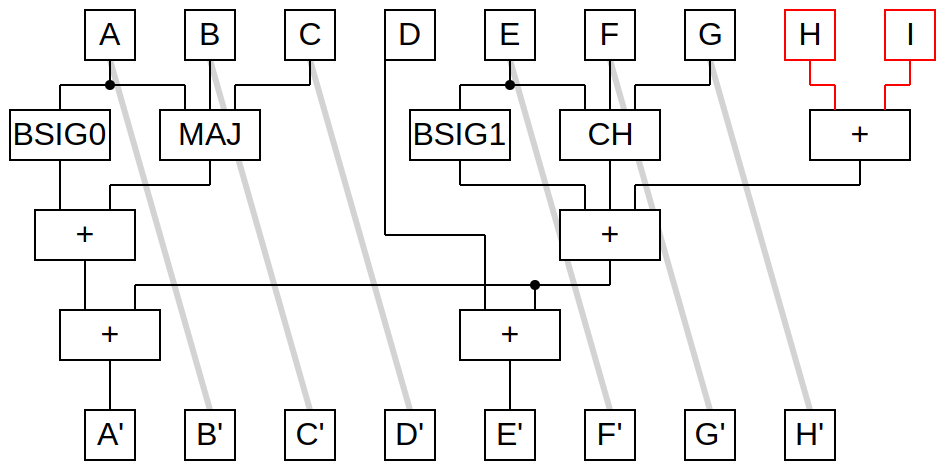
\includegraphics[width=300pt]{analyse_kern}
  \end{frame}
\end{document}